\documentclass{article}
\usepackage[margin=2cm]{geometry}

\input{./basic-tex-config/preamble.tex}

\graphicspath{{./images/}}

\title{ЛАБОЛАТОРНАЯ РАБОТА ПО КУРСУ\\ <<КВАНТОВЫЙ КОМПЬЮТЕР>>\\
Элементарные квантовые алгоритмы}
\date{Санкт-Петербург, 2017}
\author{Плотников Антон, А4101}


\begin{document}

\maketitle
\newpage

\section{Цель работы}
Изучение основных однокубитовых квантовых логических алгоритмов.

\section{Задачи}


\begin{enumerate}
  \item Изучение работы квантовых логических алгоритмов \verb|X|, \verb|Z| и 
    \verb|H|.

  \item Прогнозирование результатов виртуального эксперимента и сравнение
    результатов теоретических и экспериментальных расчетов.

  \item Распознавание неизвестного однокубитового квантового логического
    алгоритма.
\end{enumerate}

\section{Методика проведения исследования}

\begin{enumerate}
  \item Подаем кубит на вход известного логического элемента и получает
    выходной кубит. Результаты работы схемы сравниваются со свойствами
    алгоритма, известными из теории.

  \item Используя матричное представление элемента, прогнозируем результаты
    виртуального эксперимента и сравниваем результаты теоретических и
    экспериментальных расчетов.

  \item Распознаем неизвестный однокубитовый квантовый логический элемент
    \verb|X|, \verb|Z| или \verb|H|.
\end{enumerate}

\section{Анализ погрешностей}

Пусть $\ket{\phi_1}$. состояние, соответствующее первой альтернативе, а
$\ket{\phi_2}$ состояние, соответствующее второй альтернативе. Пусть перед
измерением система находилась в состоянии $c_1\ket{\phi_1} + c_2\ket{\phi_2}$.
Тогда с вероятностью $|c_1|^2$ измерение даст первый результат, и система
окажется после измерения в состоянии $\ket{\phi_1}$, а с вероятностью $|c_2|^2$
измерение даст второй результат, и система окажется после измерения в состоянии
$\ket{\phi_2}$.

Таким образом, при измерении исходного состояния $\ket\phi = 0.5\ket0
+0.86\ket1$ с вероятностью $0.25$ мы получим $\ket0$ и с вероятностью $0.7396$
--- $\ket1$.

Исходный вектор: $\ket\phi = -0.9\ket0-0.43\ket1$. В таком случае
$p(\ket0)=0.81$ и $p(\ket1)=0.1849$.

\section{Результаты}

\subsection{Исходный вектор: $\ket\phi = 0.5\ket0+0.86\ket1$}
 
\subsubsection{Оператор NOT}
 
Теоретические расчеты: $X\ket{\phi} = 0.86\ket{0}+0.5\ket{1}$
 
Экспериментальные расчеты:
 
\begin{figure}[H]
  \center{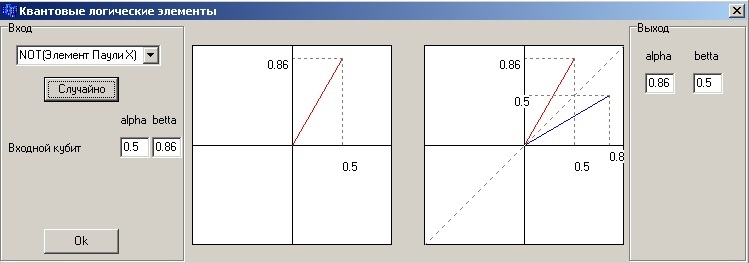
\includegraphics[width=0.85\textwidth]{NOT_1}}
\end{figure}
 
\subsubsection{Элемент Адамара}
 
Теоретические расчеты: $H\ket{\phi} =
\frac{1.36\ket{0}-0.36\ket{1}}{\sqrt{2}}\approx 0.96\ket{0}-0.25\ket{1}$
 
Экспериментальные расчеты:
 
\begin{figure}[H]
  \center{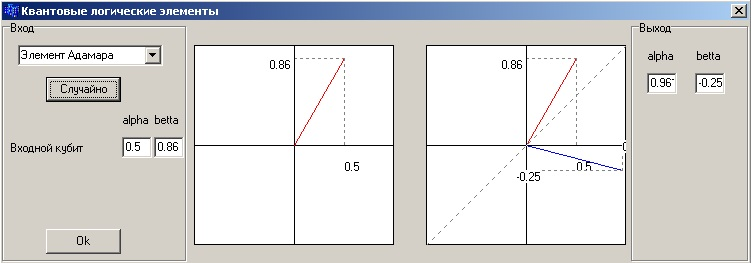
\includegraphics[width=0.85\textwidth]{H_1}}
\end{figure}
 
\subsubsection{Элемент Паули Z}
 
Теоретические расчеты: $Z\ket{\phi} = 0.5\ket{0}-0.86\ket{1}$
 
Экспериментальные расчеты:

\begin{figure}[H]
  \center{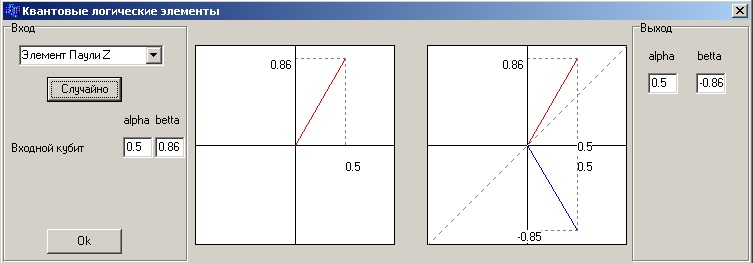
\includegraphics[width=0.85\textwidth]{Z_1}}
\end{figure}

\subsection{Матричное представление элементов}

\begin{align}
  X\begin{pmatrix} \alpha \\ \beta\end{pmatrix} &=
  \begin{pmatrix} 0 & 1 \\ 1 & 0 \end{pmatrix}
  \begin{pmatrix} 0.5 \\ 0.86 \end{pmatrix} =
  \begin{pmatrix} 0.86 \\ 0.5 \end{pmatrix}
\\
  H\begin{pmatrix} \alpha \\ \beta\end{pmatrix} &=
  \frac{1}{\sqrt2}\begin{pmatrix} 1 & 1 \\ 1 & -1 \end{pmatrix}
  \begin{pmatrix} 0.5 \\ 0.86 \end{pmatrix} =
  \frac{1}{\sqrt2}\begin{pmatrix} 1.36 \\ -0.36 \end{pmatrix}
  \approx \begin{pmatrix} 0.96 \\ -0.25 \end{pmatrix}
\\
  Z\begin{pmatrix} \alpha \\ \beta\end{pmatrix} &=
  \begin{pmatrix} 0 & 1 \\ 1 & 0 \end{pmatrix}
  \begin{pmatrix} 0.5 \\ 0.86 \end{pmatrix} =
  \begin{pmatrix} 0.5 \\ -0.86 \end{pmatrix}
\end{align}

\subsection{Исходный вектор: $\ket{\phi} = -0.9\ket{0}-0.43\ket{1}$}

Экспериментальные расчеты:

\begin{figure}[H]
  \center{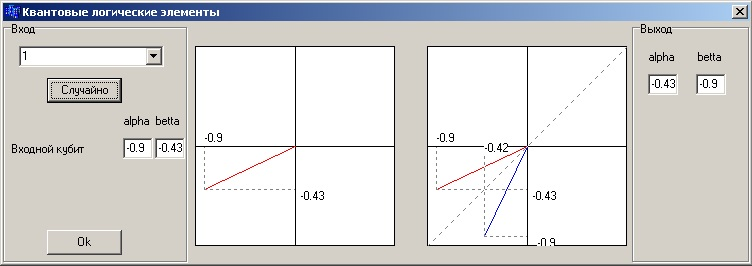
\includegraphics[width=0.85\textwidth]{1_1}}
\end{figure}

Мы видим, что в результате работы оператора коэффициенты $\alpha$ и $\beta$
меняются местами, что соответствует оператору NOT.

Экспериментальные расчеты:

\begin{figure}[H]
  \center{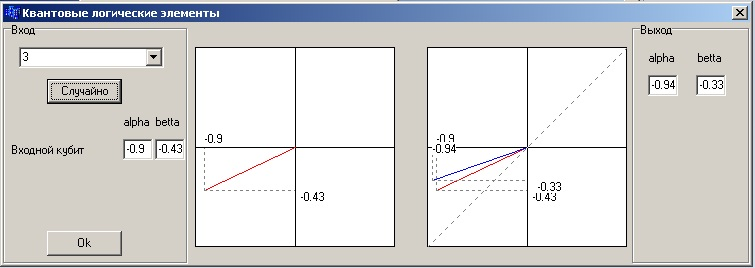
\includegraphics[width=0.85\textwidth]{3_1}}
\end{figure}

Преобразование не соответствует ни матрице X, ни Z. Убедимся, что данное
действие оператора принадлежит элементу Адамара: $H\ket{\phi} =
\frac{-1.33\ket{0}-0.47\ket{1}}{\sqrt{2}}\approx -0.94\ket{0}-0.33\ket{1}$.

Экспериментальные расчеты:

\begin{figure}[H]
  \center{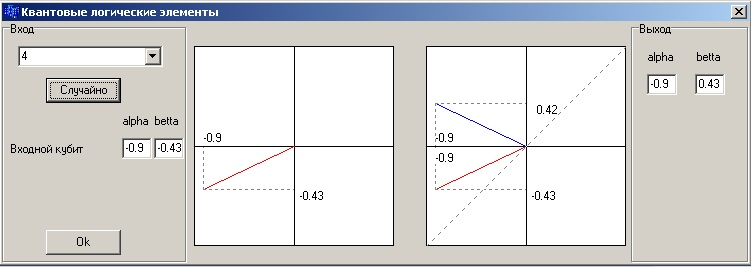
\includegraphics[width=0.85\textwidth]{4_1}}
\end{figure}

В результате работы оператора коэффициент $\alpha$ остается без изменения, в то
время как $\beta$ меняет знак. Это соответствует элементу Паули Z.\\

\section{Выводы}

Изучили работы квантовых логических алгоритмов X, Z и H. В ходе работы
сравнили теоретические экспериментальные и матричные расчеты, которые дали
одинаковый результат.

\end{document} 
